\section{Listen - x}
\subsection{Speicherung mehrerer Elemente desselben Typs}
\begin{itemize}
  \item Array: wenn die Anzahl Elemente statisch ist \\ $\rightarrow$  \lstinline{double statArray[20];} 
  \item Dynamisch allozierter Array: wenn erst zur Laufzeit die Grösse festgelegt wird, dann aber fix bleibt \\ $\rightarrow$ 
  \lstinline{double* dynArray = new double[varSize];}
  \item Liste: wenn die Anzahl Elemente erst zur Laufzeit bekannt ist und laufend ändert
\end{itemize}

\subsection{Eigenschaften einer Liste}
\begin{itemize}
  \item Eine Liste ist eine sequentielle Anordnung von Listenelementen.
  \item Die Listenelemente, auch Knoten (Node) genannt, werden miteinander mittels Pointer verbunden.
  \item Listenanfang: Muss immer gegeben sein, da von diesem ausgegangen wird. 
  \item Listenende: Muss immer gekennzeichnet werden. Wird durch Nullpointer definiert
  \item Besitzt die Grundoperationen: Element einfügen (insert), ELement löschen (delete), Element suchen (search)
\end{itemize}

\subsection{Einfach verkettete Liste - Single Linked List}
\begin{itemize}
  \item Eine einfach verkettete Liste verbindet die Listenelemente nur einfach, d.h. es gibt eine Pointerverbindung nur in eine Richtung.
\end{itemize}

\subsubsection{Definition eines Listenelementes}
\begin{flushleft}
  {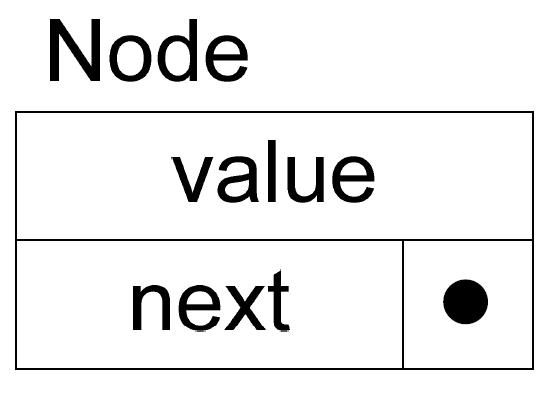
\includegraphics[width=0.1\textwidth]{images/Listen/SLL.png}}
  \label{Fig: Single Linked List}
\end{flushleft}
\lstinputlisting[language=C++]{code/Node_EinfachVerketteteListe.cpp}

\subsubsection{Bezeichnung des Listenanfangs}
\begin{flushleft}
  {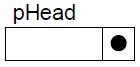
\includegraphics[width=0.1\textwidth]{images/Listen/SLL_Anfang.jpg}}
  \label{Fig: Single Linked List}
\end{flushleft}
\lstinputlisting[language=C++]{code/Listenanfang_EinfachVerketteteListe.cpp}

\subsubsection{Bezeichnung des Listenendes}
\begin{itemize}
  \item Das Listenende wird mit einem Nullpointer gekennzeichnet.
\end{itemize}
\begin{flushleft}
  {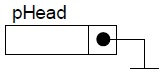
\includegraphics[width=0.15\textwidth]{images/Listen/SLL_Ende.jpg}}
  \label{Fig: Single Linked List}
\end{flushleft}

\subsubsection{Listenelement einfügen}
\begin{flushleft}
{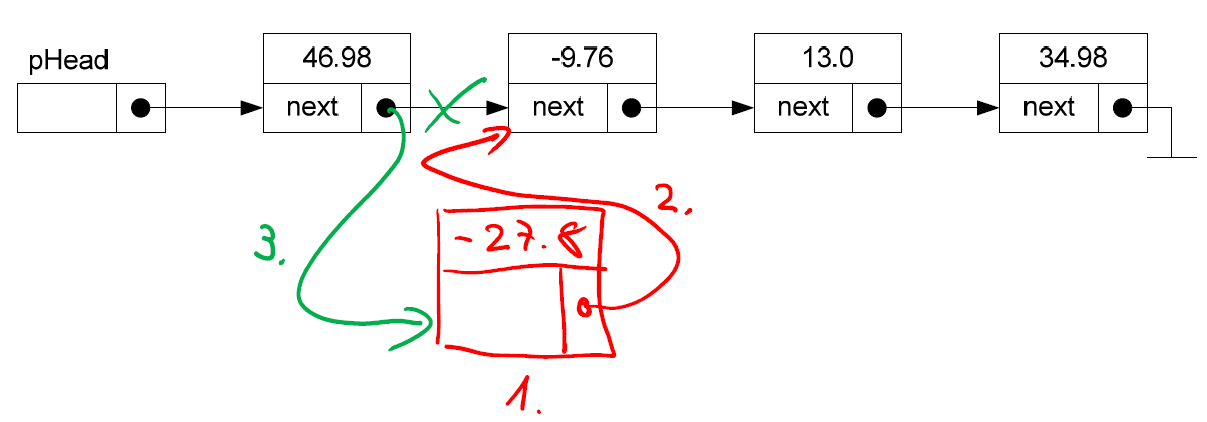
\includegraphics[width=0.5\textwidth]{images/Listen/SLL_Insert.png}}
\label{Fig: Element bei SLL einf"ugen}
\end{flushleft}
\lstinputlisting[language=C++]{code/ListenelementEinfuegen_EinfachVerketteteListe.cpp}

\subsubsection{Listenelement löschen}
\begin{flushleft}
{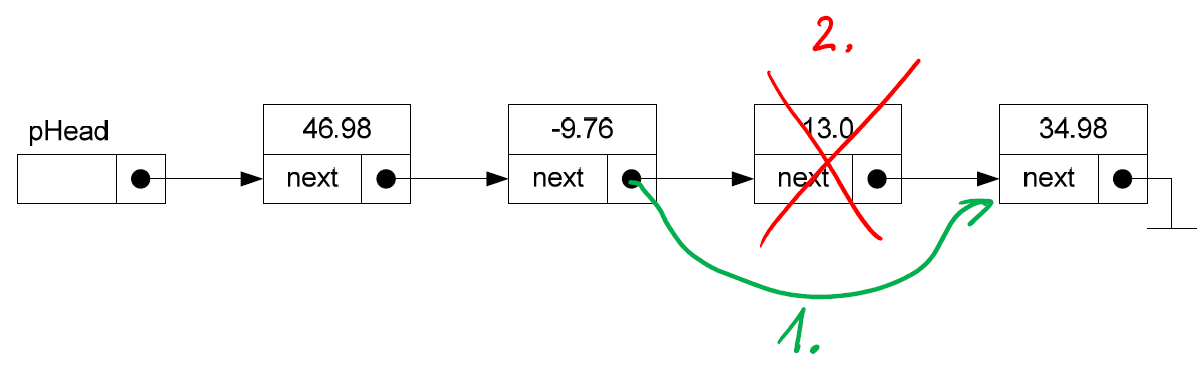
\includegraphics[width=0.5\textwidth]{images/Listen/SLL_Delete.png}}
\label{Fig: Element bei SLL l"oschen}
\end{flushleft}
\lstinputlisting[language=C++]{code/ListenelementLoeschen_EinfachVerketteteListe.cpp}

\subsubsection{Listenelement suchen}
\lstinputlisting[language=C++]{code/ListenelementSuchen_EinfachVerketteteListe.cpp}

----- BIS HIER!!!!!! ------

\subsection{Doppelt verkettete Liste - Double Linked List}
\begin{flushleft}
{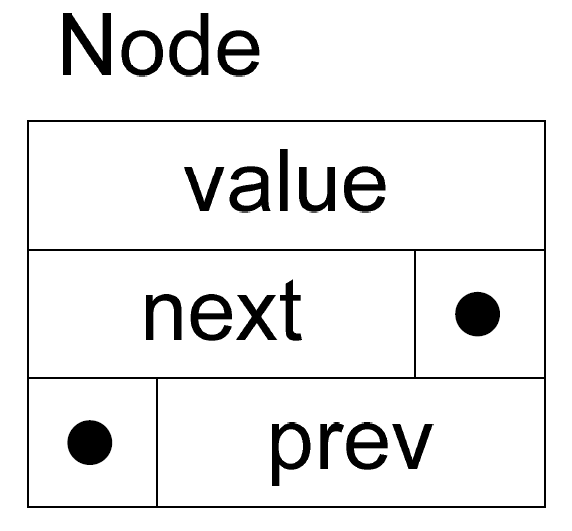
\includegraphics[width=0.1\textwidth]{images/Listen/DLL.png}}
\label{Fig: Double Linked List}
\end{flushleft}
\subsubsection{Definition Node}
\begin{lstlisting}[style=C]
struct Node
{
	Item value; // der gespeicherte Wert, z.B. double
	Node* next; // Pointer auf das naechste Listenelement
	Node* prev; // Pointer auf das vorheriges Listenelement
};
\end{lstlisting}

\subsubsection{Listenelement einf"ugen}
\begin{lstlisting}[style=C]
void DList::insertAt(int pos,double val)
{
	assert(pos >= 0);
	Node* pEl = new Node;
	pEl->value = val;
	if (pos != 0)
	{
		Node* p = nodePtr(pos);
		assert(p != 0);
		pEl->next = p->next;
		pEl->prev = p;
		p->next = pEl;
	}
	else // insert at head
	{
		pEl->next = pHead;
		pEl->prev = 0;
		pHead = pEl;
	}
	if (pEl->next != 0) // not last element in list
	{
		pEl->next->prev = pEl;
	}
	++nr;
}
\end{lstlisting}
\begin{flushleft}
{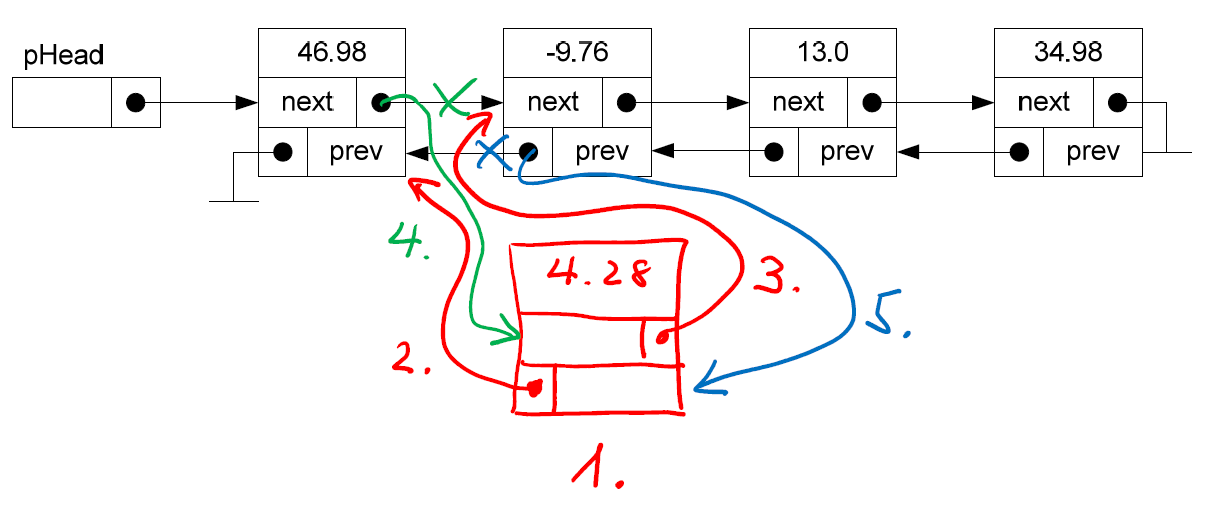
\includegraphics[width=0.5\textwidth]{images/Listen/DLL_Insert.png}}
\label{Fig: Element bei DLL einf"ugen}
\end{flushleft}

\subsubsection{Listenelement l"oschen}
\begin{lstlisting}[style=C]
void DList::deleteAt(int pos)
{
	assert(pos > 0 && pos <= nr);
	Node* pDel = nodePtr(pos); // node to be deleted
	assert (pDel != 0);
	if (pos == 1) // first element
		pHead = pHead->next;
	else
	{
		pDel->prev->next = pDel->next;
	}
	if (pDel->next != 0) // not last element in list
	pDel->next->prev = pDel->prev;
	delete pDel;
	--nr;
}
\end{lstlisting}
\begin{flushleft}
{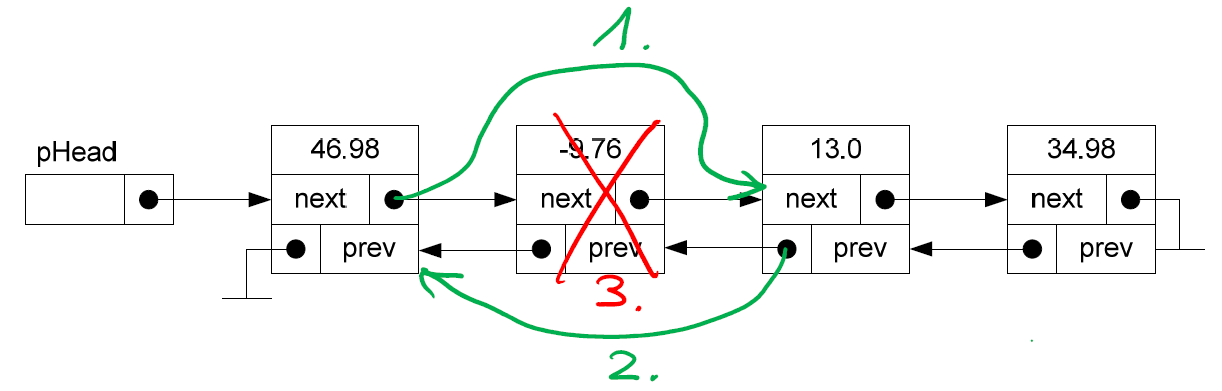
\includegraphics[width=0.5\textwidth]{images/Listen/DLL_Delete.png}}
\label{Fig: Element bei DLL l"oschen}
\end{flushleft}

\subsubsection{Listenelement suchen}
\begin{lstlisting}[style=C]
int DList::search(double val) const
{
	Node* p = pHead; // p points to element at pos 1, if not empty
	for (int i = 1; p; i++)
	{
		if (p->value == val)
		{
			return i;
		}
		p = p->next;
	}
	return 0; // not found
}
\end{lstlisting}
